\documentclass[aspectratio=169,11pt]{beamer}

% --- Język i czcionki (XeLaTeX, jak w raporcie) ---
\usepackage{fontspec}
\usepackage{polyglossia}
\setdefaultlanguage{polish}

\usepackage{graphicx}
\usepackage{booktabs}
\usepackage{amsmath}
\usepackage{xcolor}

\graphicspath{{figures/}}

% --- Motyw / kolory dopasowane do projektu ---
\usetheme{default}
\definecolor{bgreen}{HTML}{2F6B3A}
\definecolor{agreen}{HTML}{55A868}
\definecolor{uctblue}{HTML}{4C72B0}
\definecolor{heurred}{HTML}{C44E52}

\setbeamercolor{structure}{fg=bgreen}
\setbeamercolor{frametitle}{bg=bgreen,fg=white}
\setbeamercolor{title}{fg=bgreen}
\setbeamercolor{itemize item}{fg=agreen}
\setbeamercolor{itemize subitem}{fg=agreen}
\setbeamercolor{block title}{bg=agreen,fg=white}
\setbeamercolor{block body}{bg=agreen!12}
\setbeamertemplate{navigation symbols}{}
\setbeamertemplate{itemize item}{\textbullet}
\setbeamertemplate{frametitle}{%
    \nointerlineskip
    \begin{beamercolorbox}[wd=\paperwidth,ht=3.2ex,dp=1.3ex,leftskip=0.7em,rightskip=0.7em]{frametitle}%
        \usebeamerfont{frametitle}\insertframetitle%
    \end{beamercolorbox}}
\newcommand{\werdykt}[1]{\medskip\par\textbf{Hipoteza:} #1}
\setbeamertemplate{footline}{%
    \hbox{\begin{beamercolorbox}[wd=\paperwidth,ht=2.4ex,dp=1ex,leftskip=1em,rightskip=1em]{}%
    \scriptsize\color{bgreen} Breakthrough 8$\times$8 — MCTS/UCT \hfill
    \insertframenumber\,/\,\inserttotalframenumber
    \end{beamercolorbox}}}

% --- Skróty werdyktów ---
\newcommand{\falsy}{\textcolor{red!75!black}{\textbf{Odrzucona}}}
\newcommand{\ambig}{\textcolor{orange!85!black}{\textbf{Niejednoznaczna}}}
\newcommand{\partc}{\textcolor{uctblue}{\textbf{Częściowo potwierdzona}}}

\title{Zastosowanie MCTS/UCT do gry Breakthrough 8$\times$8}
\subtitle{Raport — Metody Sztucznej Inteligencji 2}
\author{Hubert Sobociński \and Sebastian Rydz}
\date{semestr letni 2025/26}

\begin{document}

{\setbeamertemplate{footline}{}\frame{\titlepage}}

% =====================================================================
\section{Wprowadzenie}

\begin{frame}{Gra Breakthrough}
    \begin{columns}[T]
    \begin{column}{0.55\textwidth}
        \begin{itemize}
            \item Gra strategiczna dwóch graczy na planszy 8$\times$8.
            \item Każdy zaczyna z dwoma rzędami pionków (16 sztuk).
            \item Ruch: do przodu lub na ukos; \textbf{bicie tylko na ukos}.
            \item \textbf{Cel:} dotrzeć pionkiem do ostatniego rzędu
                  (lub pozbawić przeciwnika ruchów).
            \item Proste reguły, ale skomplikowana \textbf{taktyka}.
        \end{itemize}
    \end{column}
    \begin{column}{0.45\textwidth}
        \centering
        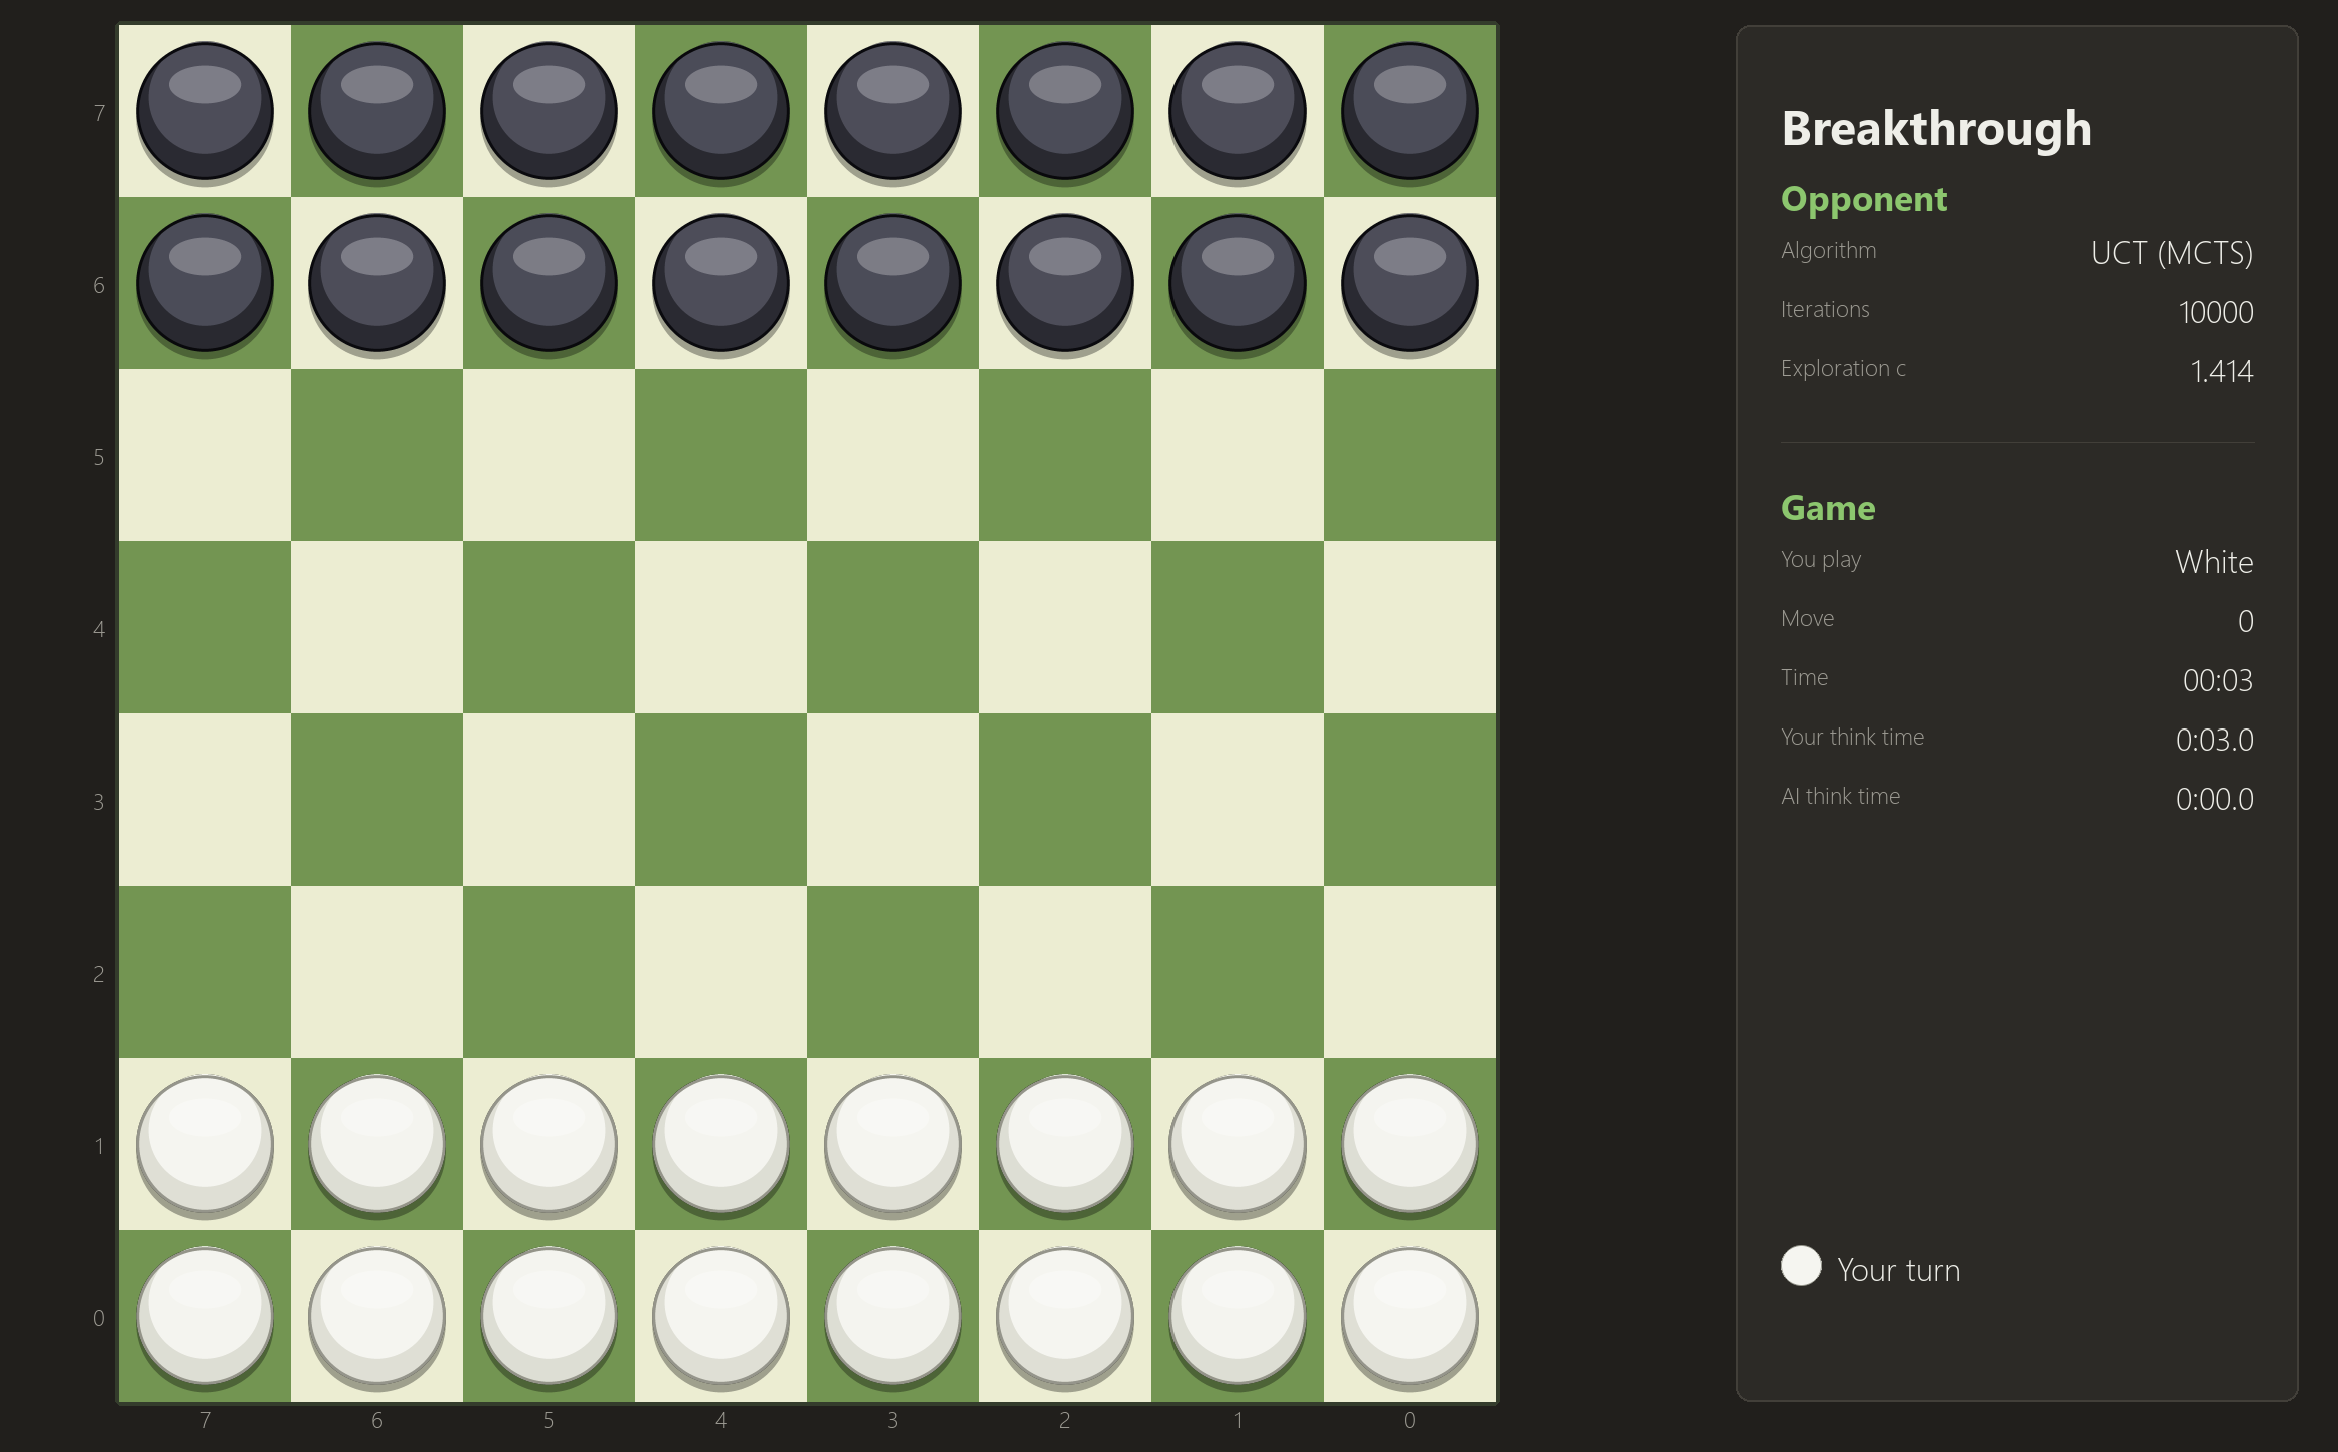
\includegraphics[width=\linewidth]{gui_2}
    \end{column}
    \end{columns}
\end{frame}

\begin{frame}{Cel projektu i pytania badawcze}
    Porównanie \textbf{MCTS/UCT} i jego rozszerzeń z klasyczną heurystyką
    alpha-beta w Breakthrough 8$\times$8. Sześć hipotez:
    \begin{itemize}
        \item \textbf{H1:} RAVE silniejszy od bazowego UCT?
        \item \textbf{H2:} Progressive Bias silniejszy od UCT?
        \item \textbf{H3:} heurystyka wygrywa przy niskim, a przegrywa przy wysokim budżecie UCT?
        \item \textbf{H4:} czy pierwszy gracz (białe) ma przewagę?
        \item \textbf{H5:} czy stała eksploracji $c$ ma wewnętrzne optimum?
        \item \textbf{H6:} czy czas decyzji rośnie w środkowej fazie gry?
    \end{itemize}
\end{frame}

% =====================================================================
\section{Metoda i implementacja}

\begin{frame}{Architektura}
    \begin{columns}[T]
    \begin{column}{0.5\textwidth}
        \textbf{Rust} — rdzeń obliczeniowy
        \begin{itemize}
            \item Bitboardy \texttt{u64} (1 bit = 1 pole).
            \item Generowanie ruchów operacjami bitowymi (maskowanie krawędzi).
            \item Hash Zobrist, klonowanie stanu w czasie stałym.
            \item Wszyscy agenci i funkcja ewaluacji.
        \end{itemize}
    \end{column}
    \begin{column}{0.5\textwidth}
        \textbf{Python 3.12} — orkiestracja
        \begin{itemize}
            \item Uruchamianie eksperymentów (multiprocessing).
            \item GUI (Pygame), analiza statystyczna.
        \end{itemize}
        \vspace{1ex}
        \textbf{Wiązanie:} PyO3 + maturin.
    \end{column}
    \end{columns}
    \vspace{1.5ex}
    \begin{block}{Dlaczego taki podział?}
        Rust daje szybkość krytyczną dla milionów symulacji MCTS, a Python —
        wygodę orkiestracji, GUI i analizy. Jeden deterministyczny generator i seedy wyprowadzane z master seeda zapewniają pełną
        reprodukowalność każdej partii.
    \end{block}
\end{frame}

\begin{frame}{Porównywane algorytmy}
    \small
    \begin{itemize}
        \item \textbf{Bazowy UCT} — MCTS bez wiedzy o grze; selekcja regułą
              UCB1:
              \[ UCT_i = \frac{w_i}{n_i} + c\sqrt{\frac{\ln N}{n_i}} \]
              \vspace{-1ex}
              \footnotesize $w_i$ — zwycięstwa, $n_i$/$N$ — odwiedziny
              węzła/rodzica, $c$ — stała eksploracji.

        \item \textbf{UCT + RAVE} — współdzielenie ocen ruchów przez statystyki
              AMAF; ocena jako średnia ważona
              $V = (1-\beta)\,V_{\text{UCT}} + \beta\,V_{\text{AMAF}}$, gdzie
              $\beta$ maleje z liczbą odwiedzin (start: AMAF $\to$ później UCT).

        \item \textbf{UCT + Progressive Bias} — wiedza heurystyczna wstrzykiwana
              do selekcji, zanikająca z odwiedzinami:
              $\text{Wartość} = UCT_i + \frac{H_i}{n_i+1}$.

        \item \textbf{Heurystyka} (minimax alfa-beta, głębokość 5) — funkcja oceny
              uwzględnia: \emph{wykładnicze zaawansowanie pionków}, groźbę
              natychmiastowego przebicia, obrońców, centralność, swobodną ścieżkę
              awansu, izolację, mobilność i przewagę materialną.
    \end{itemize}
\end{frame}

\begin{frame}{Plan eksperymentów}
    \centering
    \renewcommand{\arraystretch}{1.35}
    \small
    \begin{tabular}{c l l c}
    \toprule
     & \textbf{Co bada} & \textbf{Agenci} & \textbf{Partie} \\
    \midrule
    H1 & RAVE vs UCT & \{UCT, RAVE\} $\times$ \{5k--100k\} & 2800 \\
    H2 & Progressive Bias vs UCT & \{UCT, PB\} $\times$ \{5k--100k\} & 2800 \\
    H3 & heurystyka vs UCT & heur.\ + UCT \{500--500k\} & 4500 \\
    H4 & przewaga pierwszego gracza & UCT(5k) vs UCT(5k) & 500 \\
    H5 & strojenie stałej $c$ & UCT(10k), $c\in\{0{,}5\text{--}3\}$ & 1000 \\
    H6 & czas decyzji & UCT \{5k, 10k, 50k\} & 300 \\
    \bottomrule
    \end{tabular}

    \vspace{2ex}
    {\footnotesize Dla wszystkich: turniej każdy z każdym (100 partii na parę, 50 białymi , 50 czarnymi)}
\end{frame}

% =====================================================================
\section{Wyniki H1--H6}

\begin{frame}{H1: RAVE vs bazowy UCT}
    \begin{columns}[c]
    \begin{column}{0.62\textwidth}
        \centering
        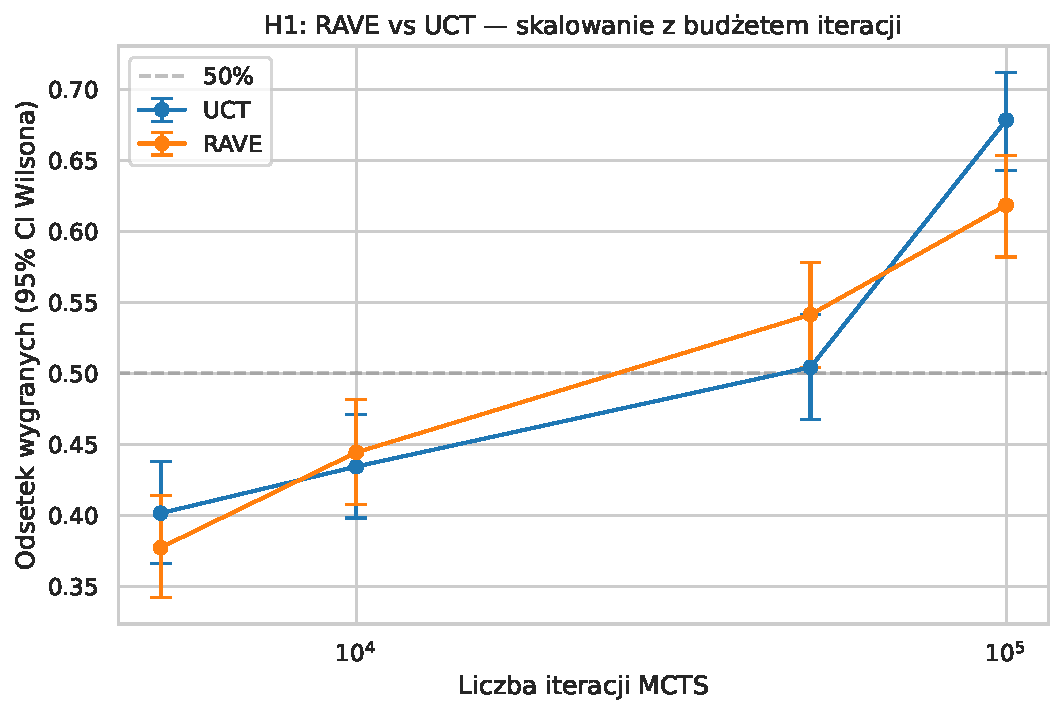
\includegraphics[width=\linewidth,height=0.74\textheight,keepaspectratio]{h1_rave_vs_uct}
    \end{column}
    \begin{column}{0.38\textwidth}
        \small
        \begin{itemize}\small
            \item Brak przewagi nad UCT; przy 100k \emph{istotnie gorszy}.
            \item AMAF zakłada przesuwalność wartości ruchu — w Breakthrough
                  to założenie się załamuje.
        \end{itemize}
        \werdykt{\falsy}
    \end{column}
    \end{columns}
\end{frame}

\begin{frame}{H2: Progressive Bias vs bazowy UCT}
    \begin{columns}[c]
    \begin{column}{0.62\textwidth}
        \centering
        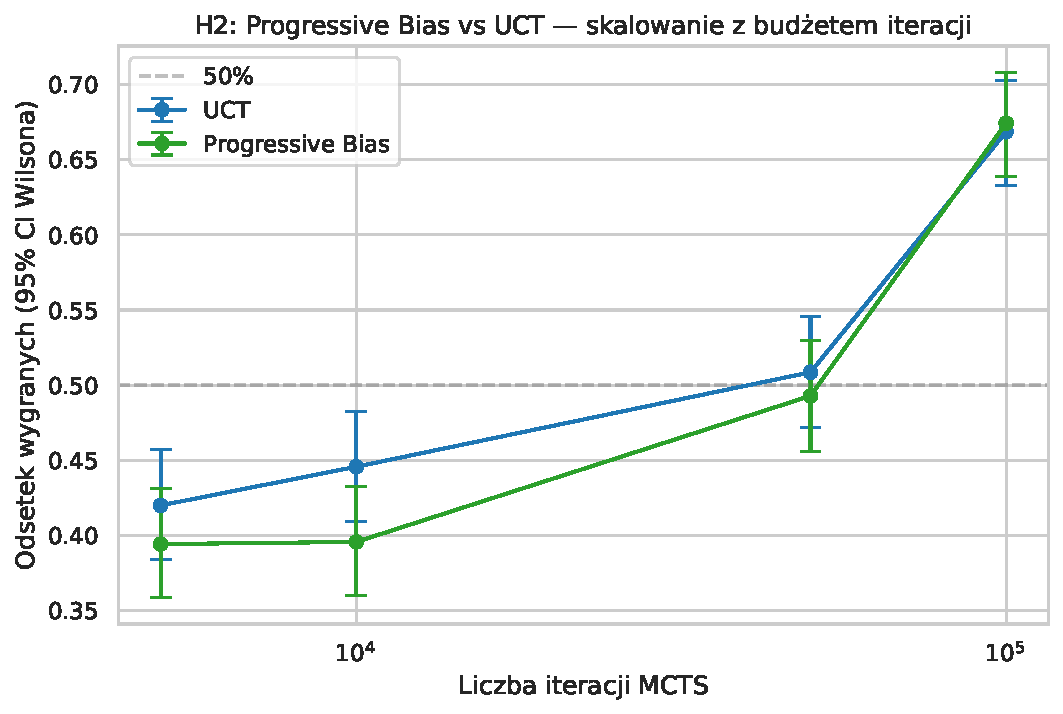
\includegraphics[width=\linewidth,height=0.74\textheight,keepaspectratio]{h2_pb_vs_uct}
    \end{column}
    \begin{column}{0.38\textwidth}
        \small
        \begin{itemize}\small
            \item Brak mierzalnej różnicy względem UCT.
            \item Wstrzykiwana wiedza domenowa jest ograniczona i zanika
                  z liczbą odwiedzin węzła.
        \end{itemize}
        \werdykt{\ambig}
    \end{column}
    \end{columns}
\end{frame}

\begin{frame}{H3: Heurystyka vs UCT}
    \begin{columns}[c]
    \begin{column}{0.62\textwidth}
        \centering
        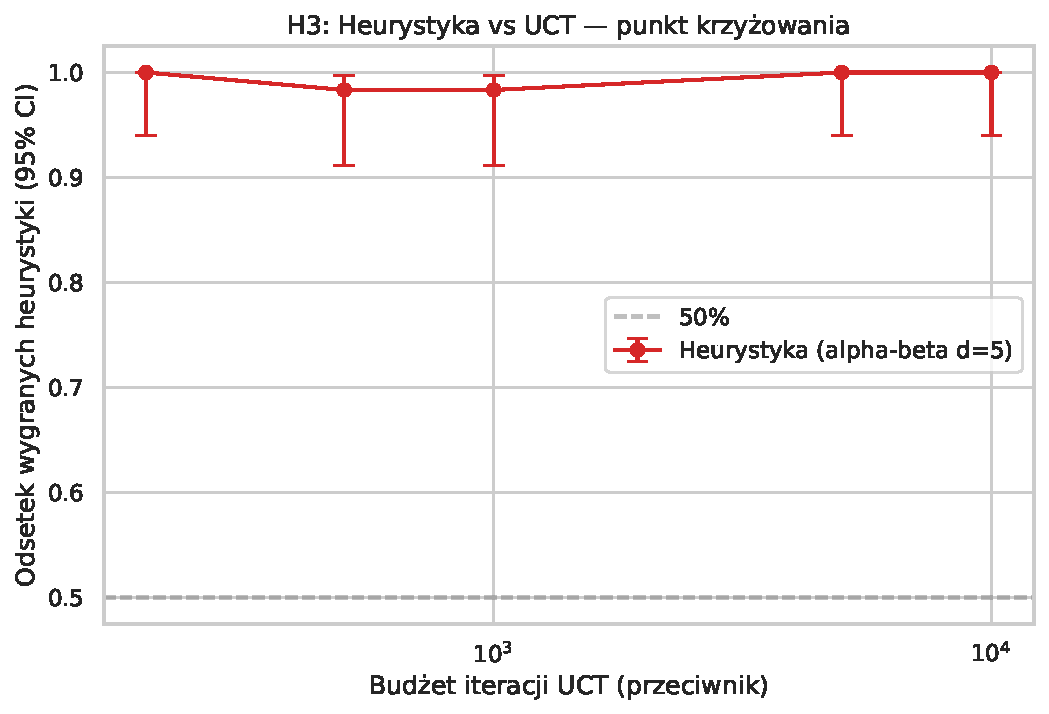
\includegraphics[width=\linewidth,height=0.74\textheight,keepaspectratio]{h3_heuristic_vs_uct}
    \end{column}
    \begin{column}{0.38\textwidth}
        \small
        Heurystyka: 100\% $\to$ 90\% przy UCT od 500 do 500k iteracji.
        \vspace{1ex}
        \begin{itemize}\small
            \item Dominuje w całym praktycznym zakresie.
            \item Nawet przy 500k iteracji (5$\times$ więcej) UCT wygrywa tylko
                  $\sim$10\% --- krzywa wypłaszcza się na $\sim$90\%,
                  \textbf{brak cross-over}.
        \end{itemize}
        \werdykt{\partc}
    \end{column}
    \end{columns}
\end{frame}

\begin{frame}{H4: Przewaga pierwszego gracza}
    \centering
    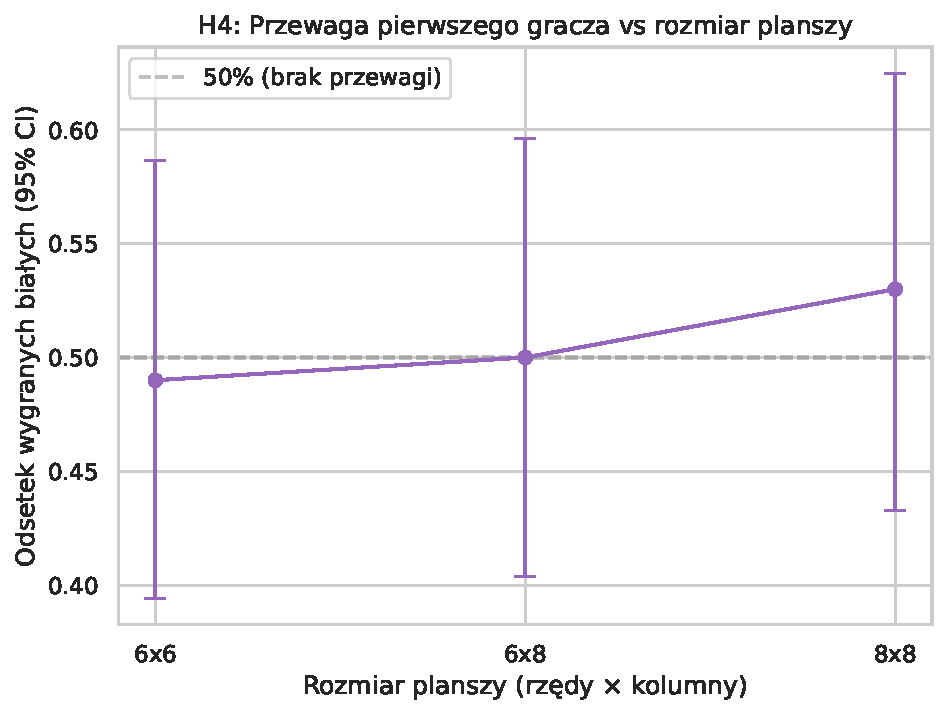
\includegraphics[width=0.92\linewidth,height=0.62\textheight,keepaspectratio]{h4_first_player_advantage}
    \\[1ex]
    \textbf{Hipoteza:} \falsy
\end{frame}

\begin{frame}{H5: Strojenie stałej eksploracji $c$}
    \begin{columns}[c]
    \begin{column}{0.55\textwidth}
        \centering
        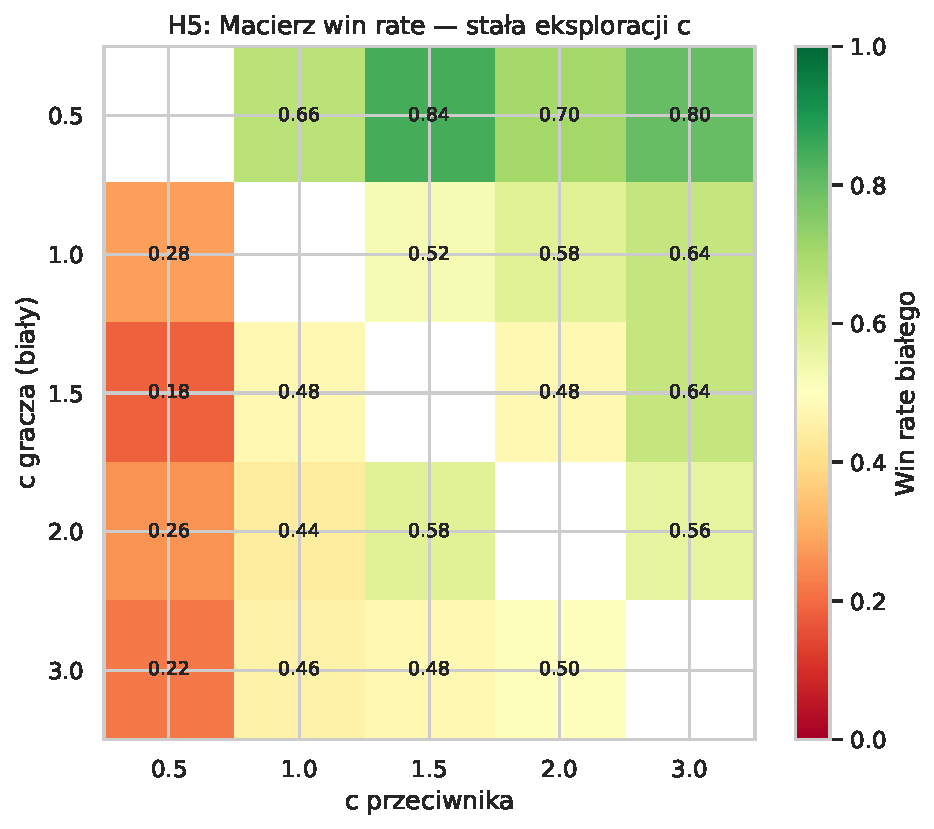
\includegraphics[width=\linewidth,height=0.76\textheight,keepaspectratio]{h5_c_heatmap}
    \end{column}
    \begin{column}{0.45\textwidth}
        \centering
        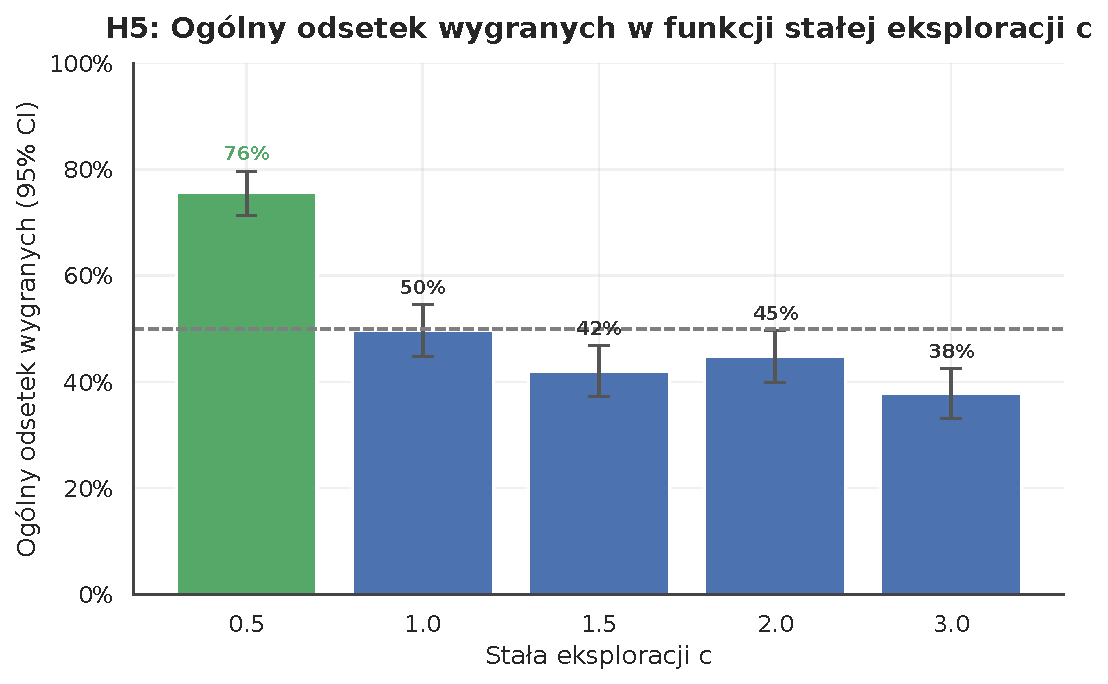
\includegraphics[width=\linewidth,height=0.48\textheight,keepaspectratio]{h5_c_bar}
        \\[0.5ex]
        \footnotesize Najlepsze $c=0{,}5$ (75,7\%), monotoniczny spadek do
        $c=3{,}0$ (37,8\%) — \textbf{brak kształtu odwróconego U}. Breakthrough
        nagradza eksploatację.
        \par\smallskip\textbf{Hipoteza:} \falsy
    \end{column}
    \end{columns}
\end{frame}

\begin{frame}{H6: Czas decyzji w trakcie partii}
    \centering
    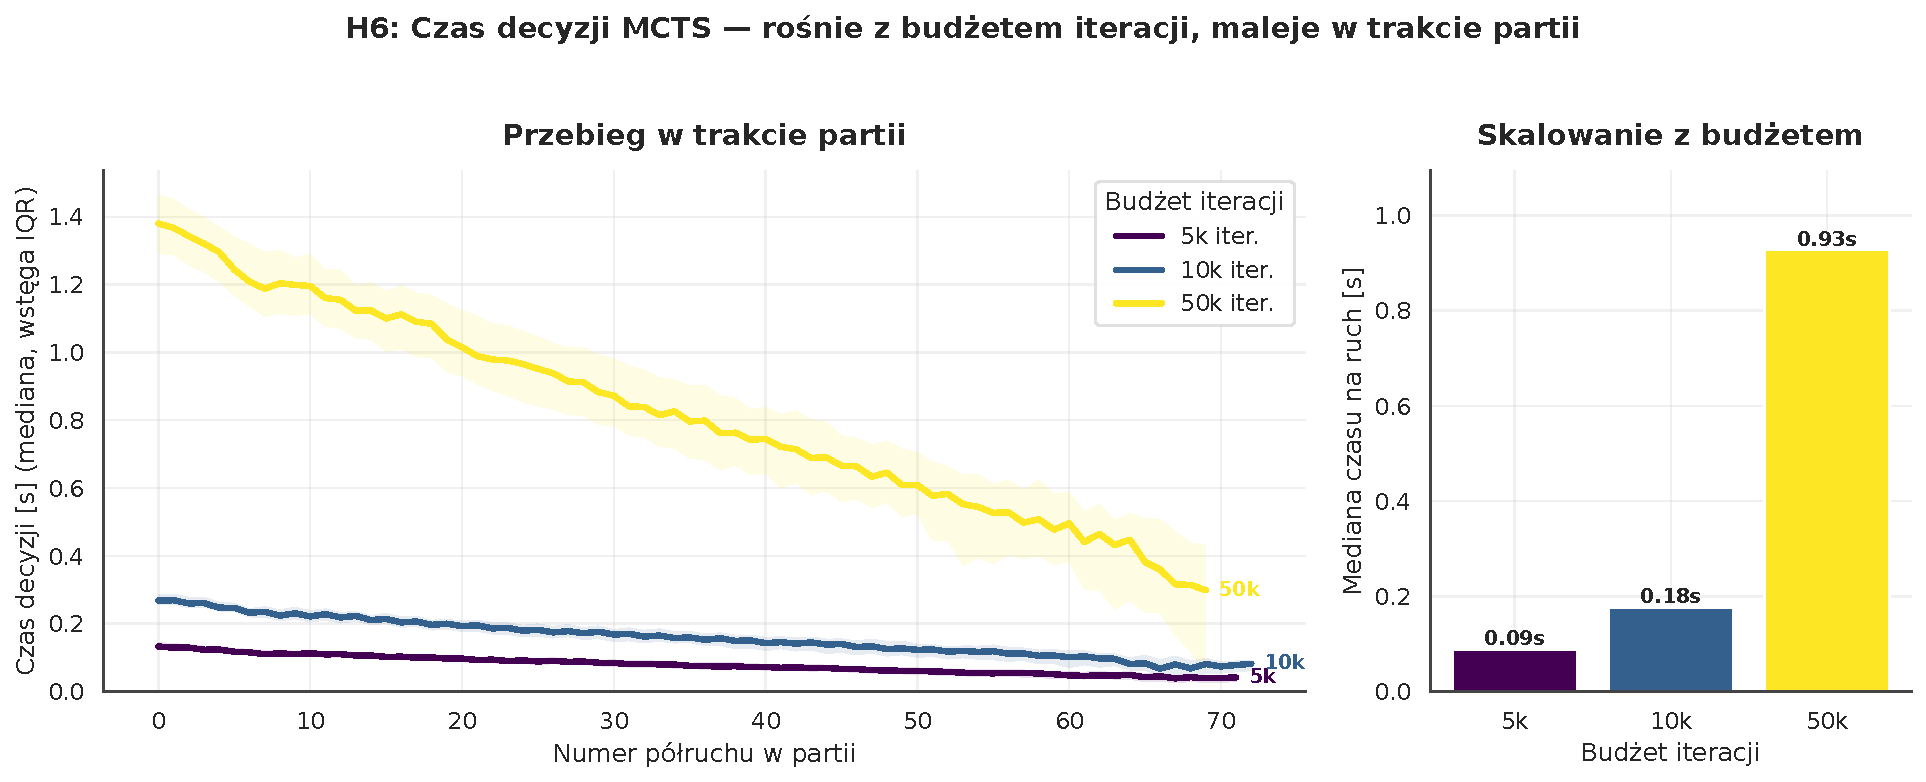
\includegraphics[width=\linewidth,height=0.64\textheight,keepaspectratio]{h6_decision_time}
    \\[0.5ex]
    \small Czas jest \emph{najwyższy w otwarciu} i maleje monotonicznie; skaluje się z budżetem: mediana 0,09 $\to$ 0,93 s (5k $\to$ 50k).
    \quad \textbf{Hipoteza:} \falsy
\end{frame}

\begin{frame}{Analizy przekrojowe (H1--H6)}
    \begin{columns}[T]
    \begin{column}{0.5\textwidth}
        \centering
        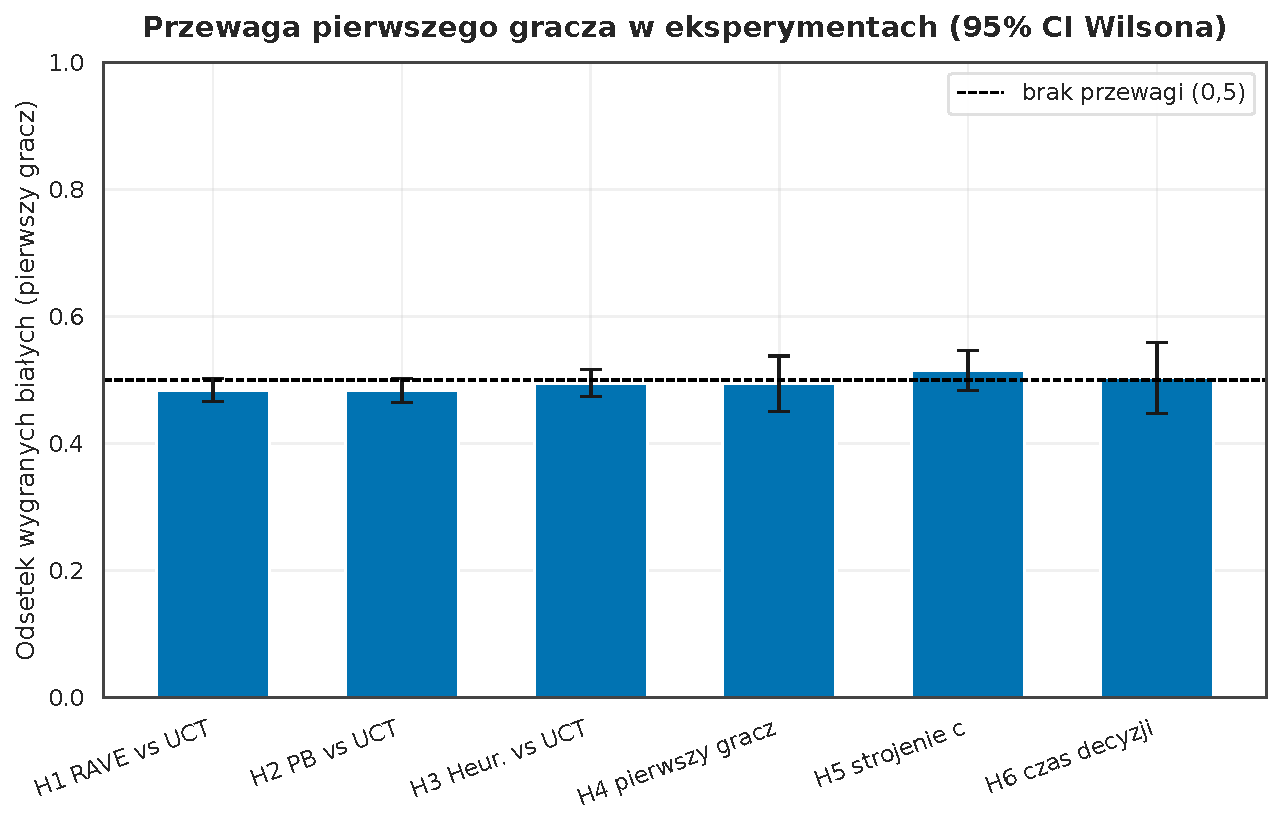
\includegraphics[width=\linewidth,height=0.62\textheight,keepaspectratio]{cross_first_player_advantage}
        \\ \footnotesize Białe 48--52\% we wszystkich eksperymentach — przewaga
        pierwszego gracza pomijalna.
    \end{column}
    \begin{column}{0.5\textwidth}
        \centering
        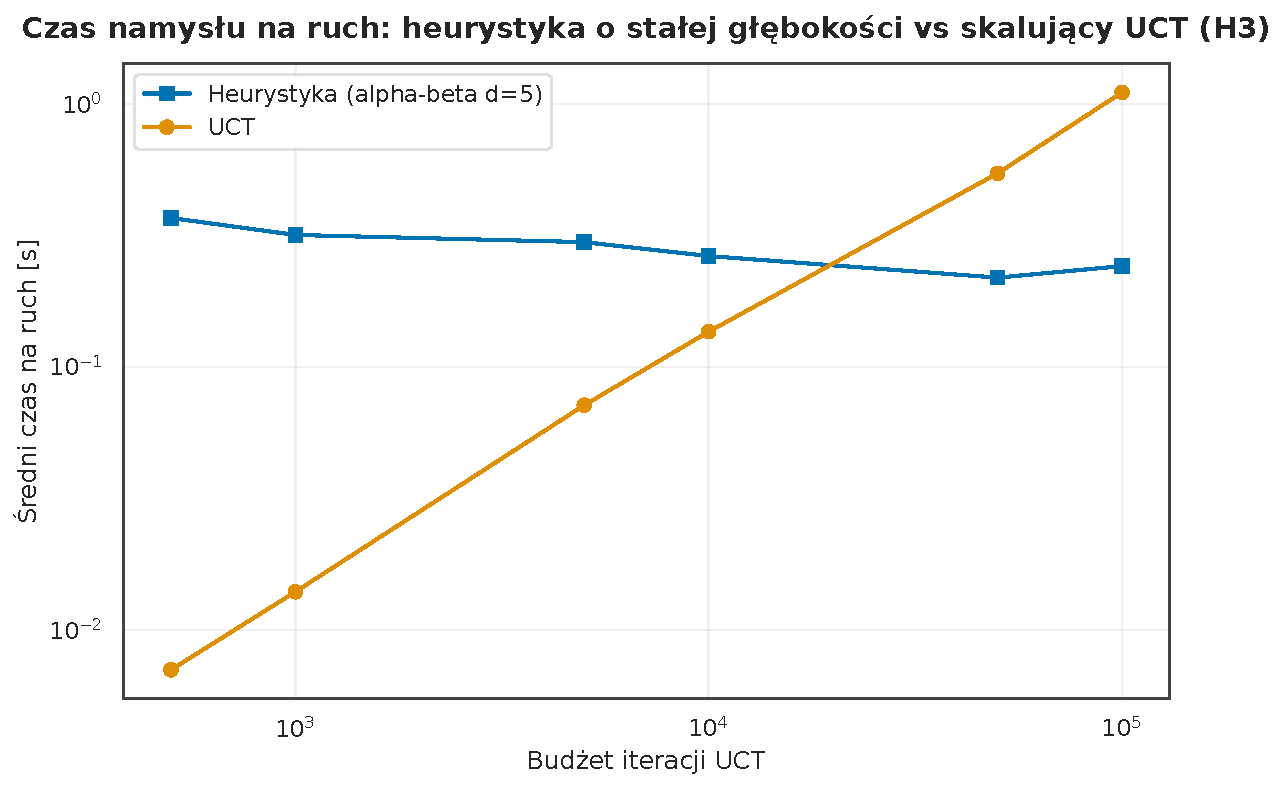
\includegraphics[width=\linewidth,height=0.62\textheight,keepaspectratio]{cross_h3_time_asymmetry}
        \\ \footnotesize UCT myśli dłużej od heurystyki dopiero $>$50k iteracji
        — a wciąż przegrywa $\geq$90\% partii (nawet przy 500k).
    \end{column}
    \end{columns}
\end{frame}

% =====================================================================
\section{Interfejs i partie z ludźmi}

\begin{frame}{Interfejs graficzny (człowiek vs AI)}
    \begin{columns}[c]
    \begin{column}{0.42\textwidth}
        \centering
        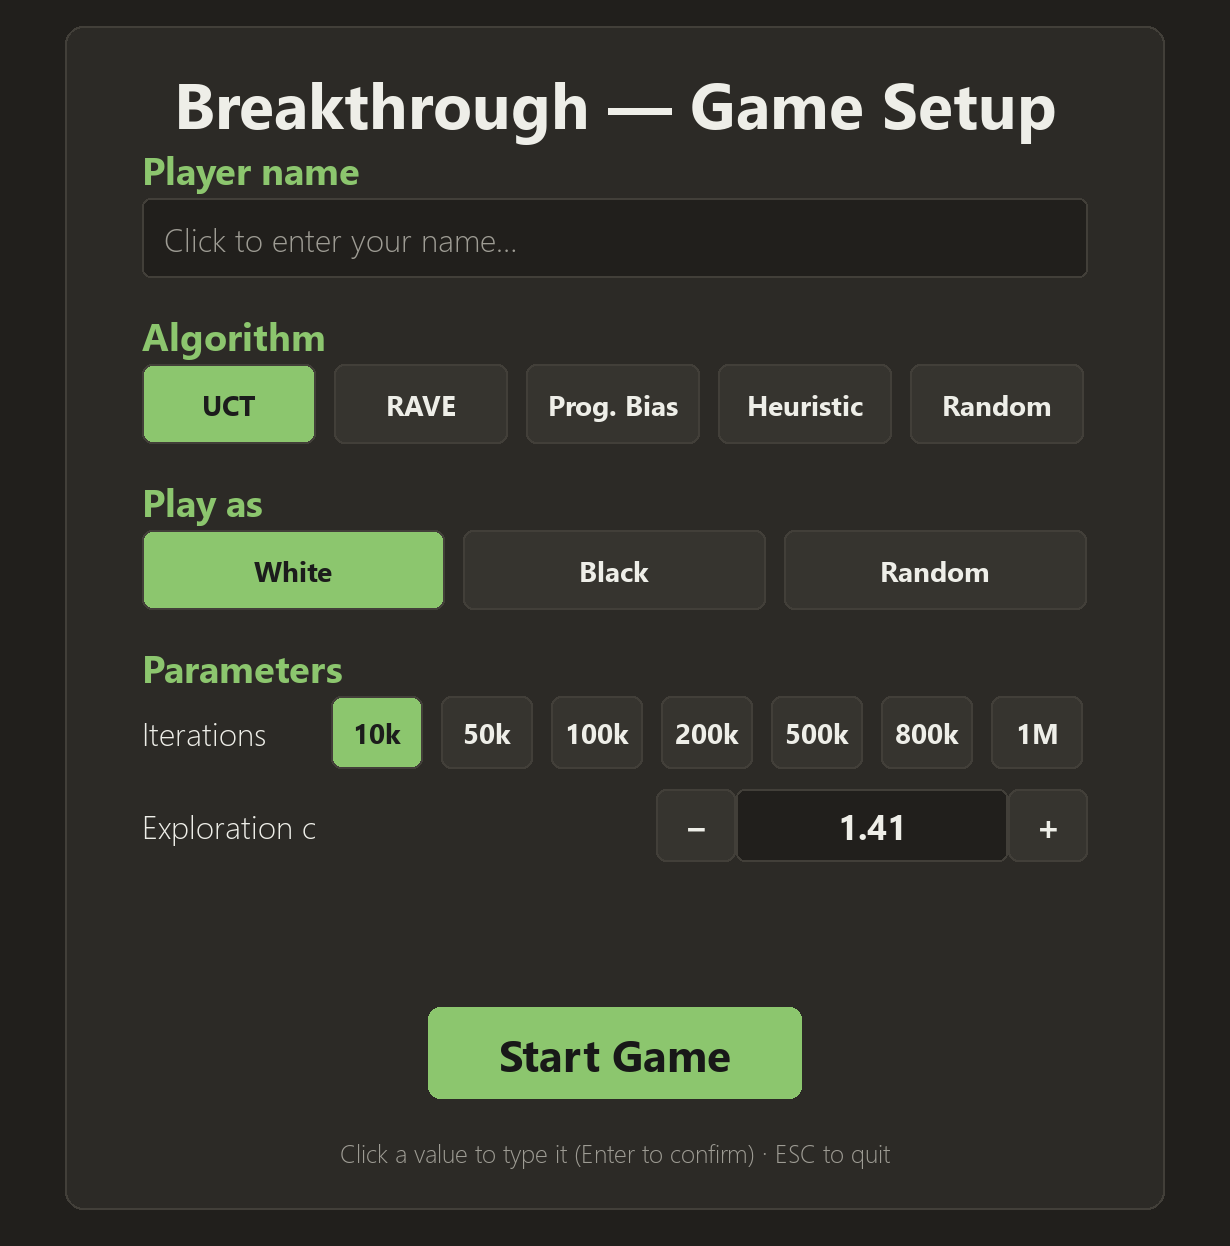
\includegraphics[height=0.80\textheight,keepaspectratio]{gui_1}
    \end{column}
    \begin{column}{0.58\textwidth}
        \centering
        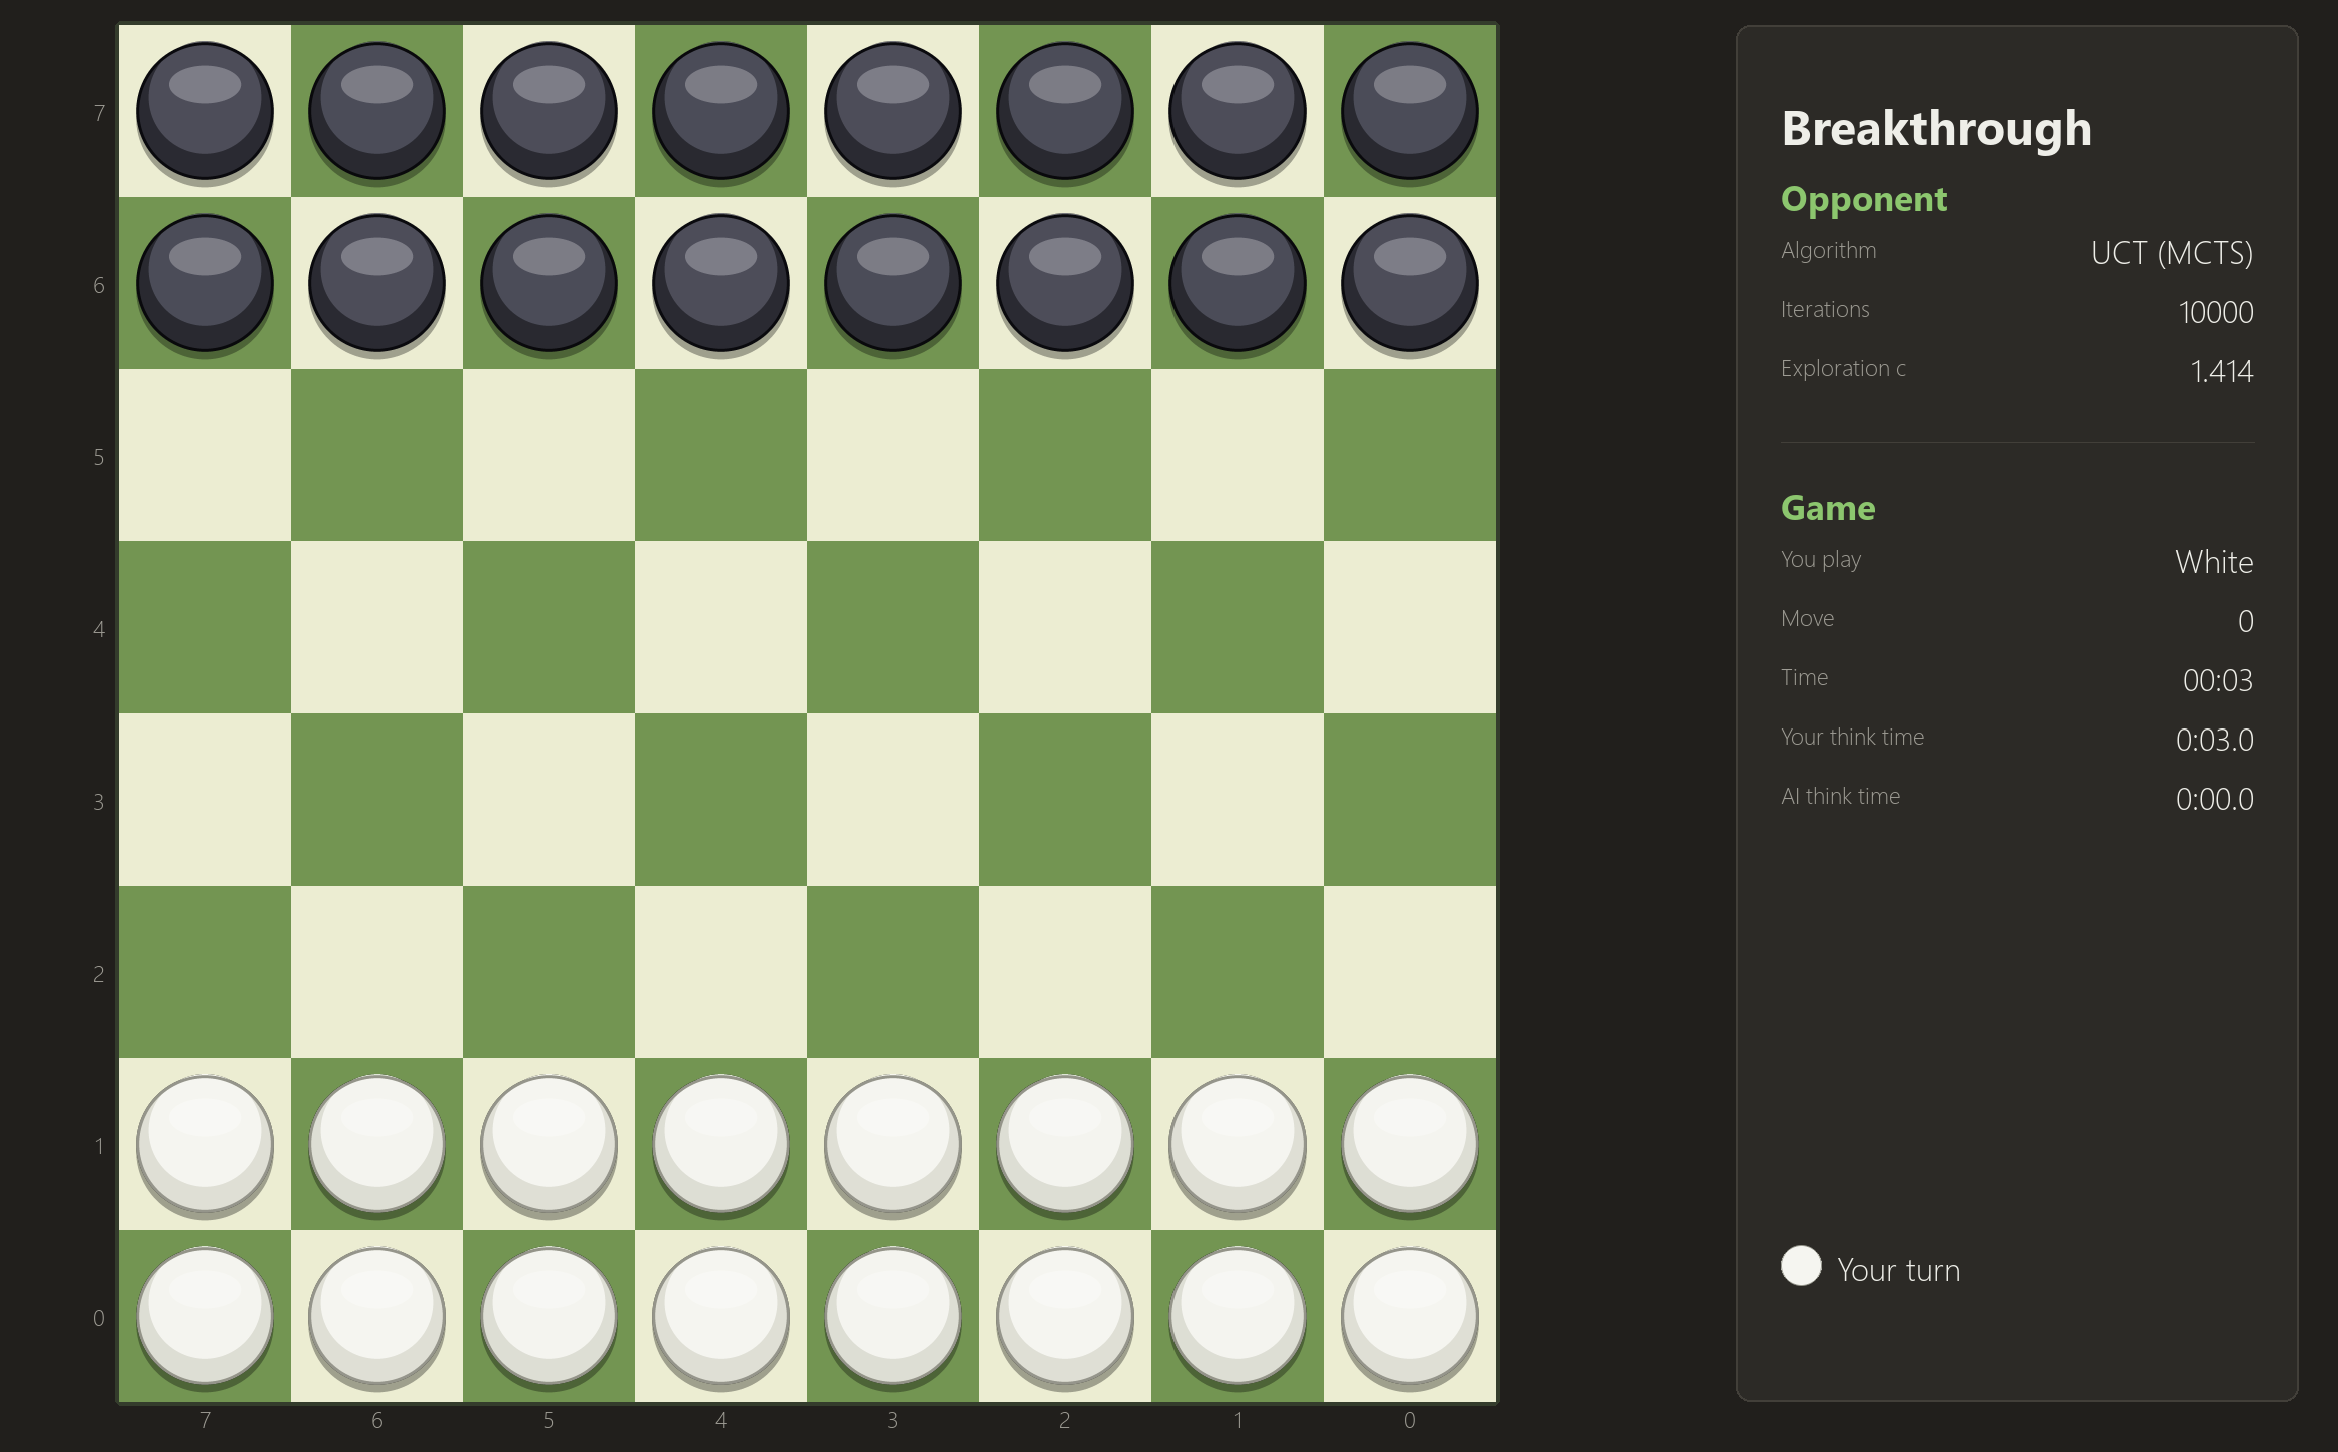
\includegraphics[width=\linewidth,keepaspectratio]{gui_2}
        \\[1ex]
        \footnotesize Wybór algorytmu, koloru i parametrów; podświetlanie
        legalnych ruchów, panel statystyk na żywo, zapis partii i oceny trudności.
    \end{column}
    \end{columns}
\end{frame}

\begin{frame}{Partie człowiek vs AI}
    \begin{columns}[c]
    \begin{column}{0.55\textwidth}
        \centering
        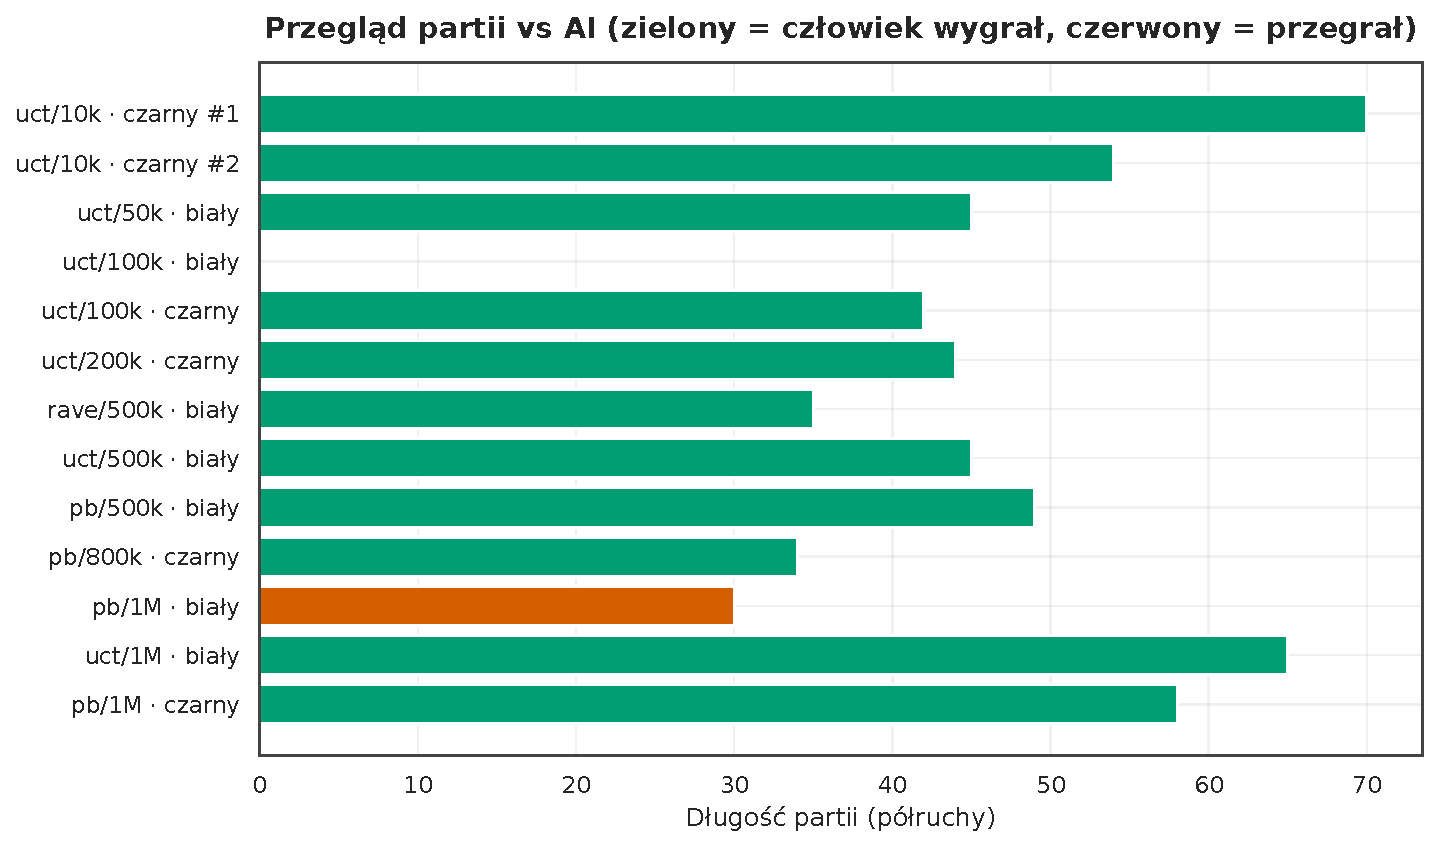
\includegraphics[width=\linewidth,height=0.74\textheight,keepaspectratio]{human_outcome_per_game}
    \end{column}
    \begin{column}{0.45\textwidth}
        \small (demonstracja narzędzia, 12 partii — nie pomiar statystyczny)
        \begin{itemize}\small
            \item Człowiek wygrał \textbf{11 z 12} partii (budżety 10k--1M).
            \item Postrzegana trudność: mediana 4,5/10.
            \item Czas AI rośnie z budżetem — do kilkudziesięciu s/ruch przy 1M.
        \end{itemize}
    \end{column}
    \end{columns}
\end{frame}

% =====================================================================
\section{Podsumowanie}

\begin{frame}{Wnioski}
    \begin{itemize}
        \item \textbf{Kluczowe odkrycie:} RAVE jest nieskuteczny w Breakthrough
              8$\times$8 — standardowe rozszerzenie MCTS z domeny Go nie przenosi
              się: wartość ruchu silnie zależy od kontekstu, więc sygnał AMAF działa słabo.
        \item Prosta \textbf{heurystyka alpha-beta dominuje} MCTS w całym
              praktycznym zakresie — jednocześnie silniejsza i tańsza.
        \item \textbf{Niski $c$} (nacisk na eksploatację) jest najlepszy —
              gra premiuje konkretne, wymuszone warianty.
        \item Brak istotnej przewagi pierwszego gracza przy MCTS o zbliżonej sile.
        \item Wniosek ogólny: w grach \emph{taktycznych} o umiarkowanym branching
              factor wiedza domenowa bije ,,zwykłe'' samplowanie MCTS.
    \end{itemize}
\end{frame}

\begin{frame}[plain]{}
    \centering
    \vfill
    {\Huge \color{bgreen}\textbf{Dziękujemy za uwagę}}\\[2ex]
    {\large Pytania?}\\[3ex]
    {\small Hubert Sobociński \quad·\quad Sebastian Rydz}
    \vfill
\end{frame}

\end{document}
